%%%%%%%%%%%%%%%%%%%%%%%%%%%%%%%%%%%%%%%%%%%%%%%%%%%%%%%%%%%%%%%%%%%%%%%%%%%%%%%%
% Template for USENIX papers.
%
% History:
%
% - TEMPLATE for Usenix papers, specifically to meet requirements of
%   USENIX '05. originally a template for producing IEEE-format
%   articles using LaTeX. written by Matthew Ward, CS Department,
%   Worcester Polytechnic Institute. adapted by David Beazley for his
%   excellent SWIG paper in Proceedings, Tcl 96. turned into a
%   smartass generic template by De Clarke, with thanks to both the
%   above pioneers. Use at your own risk. Complaints to /dev/null.
%   Make it two column with no page numbering, default is 10 point.
%
% - Munged by Fred Douglis <douglis@research.att.com> 10/97 to
%   separate the .sty file from the LaTeX source template, so that
%   people can more easily include the .sty file into an existing
%   document. Also changed to more closely follow the style guidelines
%   as represented by the Word sample file.
%
% - Note that since 2010, USENIX does not require endnotes. If you
%   want foot of page notes, don't include the endnotes package in the
%   usepackage command, below.
% - This version uses the latex2e styles, not the very ancient 2.09
%   stuff.
%
% - Updated July 2018: Text block size changed from 6.5" to 7"
%
% - Updated Dec 2018 for ATC'19:
%
%   * Revised text to pass HotCRP's auto-formatting check, with
%     hotcrp.settings.submission_form.body_font_size=10pt, and
%     hotcrp.settings.submission_form.line_height=12pt
%
%   * Switched from \endnote-s to \footnote-s to match Usenix's policy.
%
%   * \section* => \begin{abstract} ... \end{abstract}
%
%   * Make template self-contained in terms of bibtex entires, to allow
%     this file to be compiled. (And changing refs style to 'plain'.)
%
%   * Make template self-contained in terms of figures, to
%     allow this file to be compiled. 
%
%   * Added packages for hyperref, embedding fonts, and improving
%     appearance.
%   
%   * Removed outdated text.
%
%%%%%%%%%%%%%%%%%%%%%%%%%%%%%%%%%%%%%%%%%%%%%%%%%%%%%%%%%%%%%%%%%%%%%%%%%%%%%%%%

\documentclass[letterpaper,twocolumn,10pt]{article}
\usepackage{usenix2019_v3}

% to be able to draw some self-contained figs
\usepackage{tikz}
\usepackage{amsmath}

% inlined bib file
\usepackage{filecontents}
\raggedbottom

\usepackage{graphicx}
\usepackage{float}
\graphicspath{ {../images/}}

%-------------------------------------------------------------------------------
\begin{filecontents}{\jobname.bib}
%-------------------------------------------------------------------------------

\end{filecontents}

%-------------------------------------------------------------------------------
\begin{document}
%-------------------------------------------------------------------------------

%don't want date printed
\date{}

% make title bold and 14 pt font (Latex default is non-bold, 16 pt)
\title{\Large \bf The RISC Takers:\\
  Final Report}

%for single author (just remove % characters)
\author{
  {\rm Sean Keever} \\
  swkeever@uw.edu
  \and
  {\rm Yokesh Jayakumar} \\
  karthj@uw.edu
  \and
  {\rm John McMahon} \\
  mcmahjoh@uw.edu
  % copy the following lines to add more authors
  % \and
  % {\rm Name}\\
  %Name Institution
} % end author

\maketitle

%-------------------------------------------------------------------------------
\begin{abstract}
  %-------------------------------------------------------------------------------
  The goal of our project is to create a means of letting a user not only use an OS,
  but to allow a user to see what is going on inside the OS and CPU.
  To this end, our project aims to maximize availability to users by
  providing a browser-based interface that lets the user visit a webpage and
  visualize an OS from the moment he or she visits the page.
\end{abstract}

%-------------------------------------------------------------------------------
\section{Introduction}
%-------------------------------------------------------------------------------

There are multiple implementations of operating systems made available via a web
browser. Instead of re-implementing that functionality, we chose to find a project that
has the low-level emulation from C to JavaScript already handled. This way, we can
focus on solving a new problem: providing an interface to
visualize the OS and CPU.

We looked at multiple different OS implementations and decided on risv-angel,
which seemed to offer the
functionality we needed without too much underlying complexity. This way, we could
focus more attention to creating the visualization layers without having to worry
too much about the low-level emulation details.

%-------------------------------------------------------------------------------
\section{Initial Design}
%-------------------------------------------------------------------------------

To start, we stripped the riscv-angel project to only show the Terminal.
We got rid of all the elements and libraries that were not going to be used in our project.
Before we started on our implementation, we prototyped the UI in Figma, shown in Figure \ref{fig:proto1}.

\begin{figure}[H]
  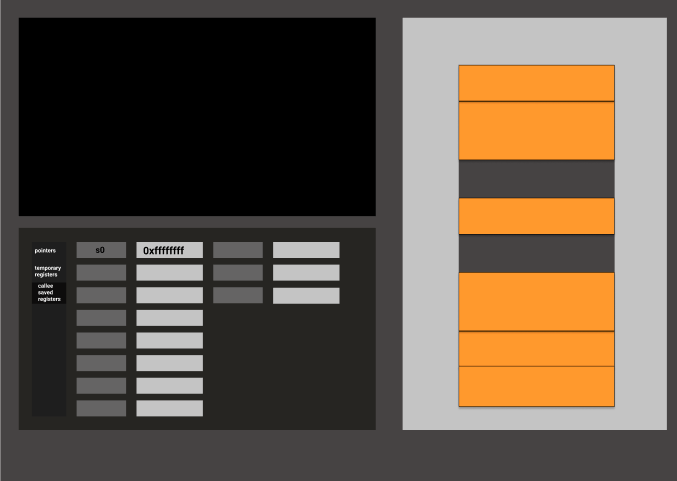
\includegraphics[scale=0.4]{prototype1}
  \caption{Initial prototype of design}
  \label{fig:proto1}
  \centering
\end{figure}

Figma allowed us to come up with a design before we implement anything in code.
We aimed for a dashboard-like interface, showing the user
information about the CPU and OS in real-time.

%-------------------------------------------------------------------------------
\section{Beginning Development}
%-------------------------------------------------------------------------------

\subsection*{Setting up a development environment}

One of the challenges for the team was facing ambiguity in this project.
It was difficult to interpret exactly what needed to be done.

To facilitate this problem and make development easier,
we started approaching the project with an Agile workflow.
We are using GitHub's Kanban board functionality to track issues and milestones.
We hold weekly stand-ups to find out

\begin{itemize}
  \item what we did over the past week, and
  \item what we will do in the next week.
\end{itemize}

\noindent
We use the GitHub issues that we created to assign tasks for each member of a group.
In doing this, we were able to be more productive by having concrete milestones in place
in order to complete the project.

To ensure robustness and quality of our project,
we have also developed some tooling for continuous integration.
To ensure consistency in the codebase, we use ESLint, a tool that we have configured
to apply the rules defined in AirBnB's style guide.
We use \texttt{lint-staged} to run our linters before any commit. This way,
we know if stylistic errors need to be addressed before pushing code to the repository.

We also set up GitHub Actions, which are essentially hooks that execute when
code is pushed to the repository.
These hooks will run the style checker and our unit tests before code is pushed to remote.
The hook will reject any commits if any of these actions fail.
The GitHub Actions are certainly overkill for our case, but we wanted to have the infrastructure
in place in order to configure our CI easily.

\subsection*{Choosing technologies}

We want our interface to be interactive, so we chose React.js as our library of choice,
which offers a means of rapidly developing interactive client-side applications.

This doesn't come without its challenges, though. The existing project uses vanilla JavaScript
in order to run the emulator. The legacy code accomplishes this by spawning a worker thread
that handles all the emulation tasks. The main thread interacts with this worker thread via
message passing.

Working with the existing riscv-angel codebase was challenging. We resolved
the issues by having rendering each dashboard component separately. This way,
the dashboard components can coexist with the existing riscv-angel project code
easily.


%-------------------------------------------------------------------------------
\section{Establishing a Design System}
%-------------------------------------------------------------------------------

None of the members on our team are trained designers. We had to be resourceful
to learn some of the patterns of good UI design. To make this easier, we took
a lot of inspiration from professionals by using the \href{https://material.io/design}{Material Design}
system used and maintained at Google. We imported a Material Design kit into Figma,
which includes many Material Design assets such as buttons, cards, etc. Doing so
allowed us to wireframe a UI prototype that we feel was closer to our vision for the app's design.
Figure \ref{fig:proto2} shows the first steps of prototyping our UI using Material Design and Figma.

\begin{figure}[H]
  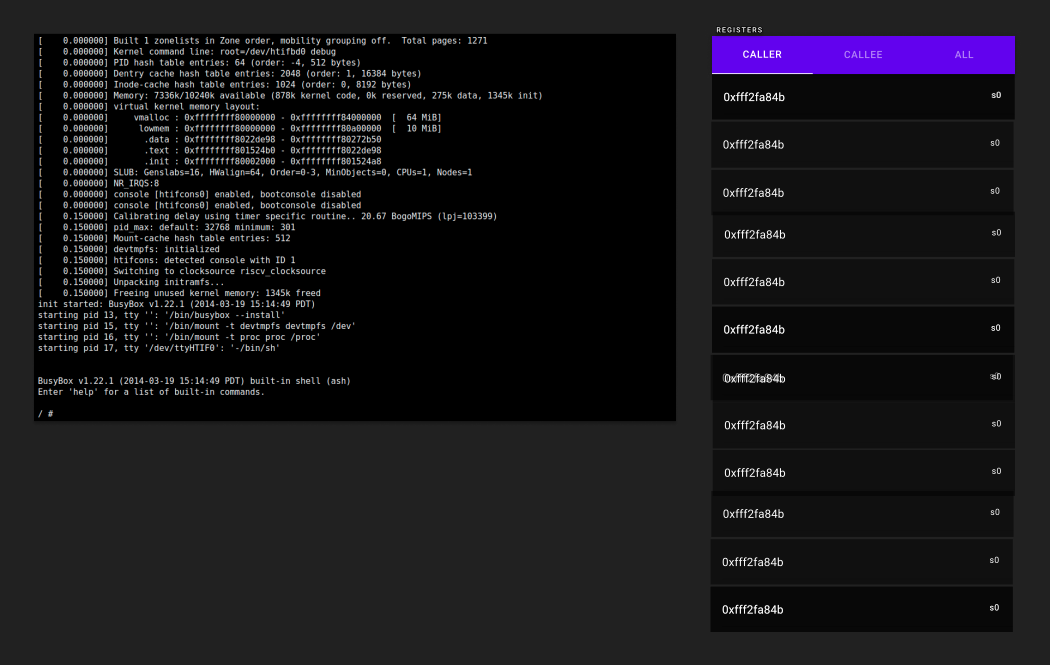
\includegraphics[scale=0.26]{prototype2}
  \caption{Initial prototype using Material Design}
  \label{fig:proto2}
  \centering
\end{figure}

In addition to our team not being expert designers, we are also not experts in CSS, which
is vital to making the application look good. We wanted our application to be as
lightweight as possible, so we wanted to have our own custom CSS, as opposed to using a CSS
framework like Bootstrap. To learn CSS and UI design
patterns further, we read the book \href{https://refactoringui.com/}{Refactoring UI}, which
provided many design tips from a developer's point of view.

We established a design system that is used throughout the app. We defined a system for colors,
fonts, spacing/font size, and more. The system restricts properties of the UI to follow a discrete
set of values. Although at first glance, it may seem that this restriction would limit our ability
to create a design. In fact, the restriction provided by the design system helped to make
the application feel polished and consistent.


%-------------------------------------------------------------------------------
\section{Implementing a Working Prototype}
%-------------------------------------------------------------------------------

\subsection*{A Modular Design}

We describe our app as a modular, dashboard user interface that lets users use a
basic OS and see properties about the OS and CPU in real time.

Our modular design means we have separate components for each visualization in the dashboard.
For example, there is a separate component for the window showing the registers, a separate
component for the view showing the ratio of instructions being executed, and so forth.
We split our app into modular components for several reasons:

\begin{itemize}
  \item easier to maintain and test
  \item allows features to rapidly developed
  \item offers more flexibility in UI structure
\end{itemize}

We will elaborate on each of these points.

First, because our dashboard interface uses modular UI components, whenever we work on a single
component, we can be confident that breaking a single component won't break other parts of the app.

The modular design also allows us to split the work and develop features independently. This is great for
us during these times of quarantine because of COVID-19. So, for example, while one team member is working on some feature
$A$, another team member can be styling feature $B$. And since the components are modular, we can do so without
worrying about conflicting with another person's work.

Finally, having the components act as modular entities allows us to change the layout of the UI very easily should
we choose too. The components are simply independent building blocks that can be moved around as we please. This
flexibility will become very important when it comes time to finalizing our app.

\subsection*{Finishing our Prototype}

Information about the CPU state lives in the existing \texttt{riscv-angel} code, which is written in
vanilla JavaScript. To pass information about the CPU to React, we bind a JavaScript object from the
\texttt{riscv-angel} code
to the globally accessible \texttt{window} object.

We then create a custom React hook that safely retrieves this state to be used by React.
With the state of the CPU accessible in our React components, we could implement our
dashboard.

In our app, we show the contents of the 32 user registers,

% change this when we have a picture of the prototype
\begin{figure}[H]
  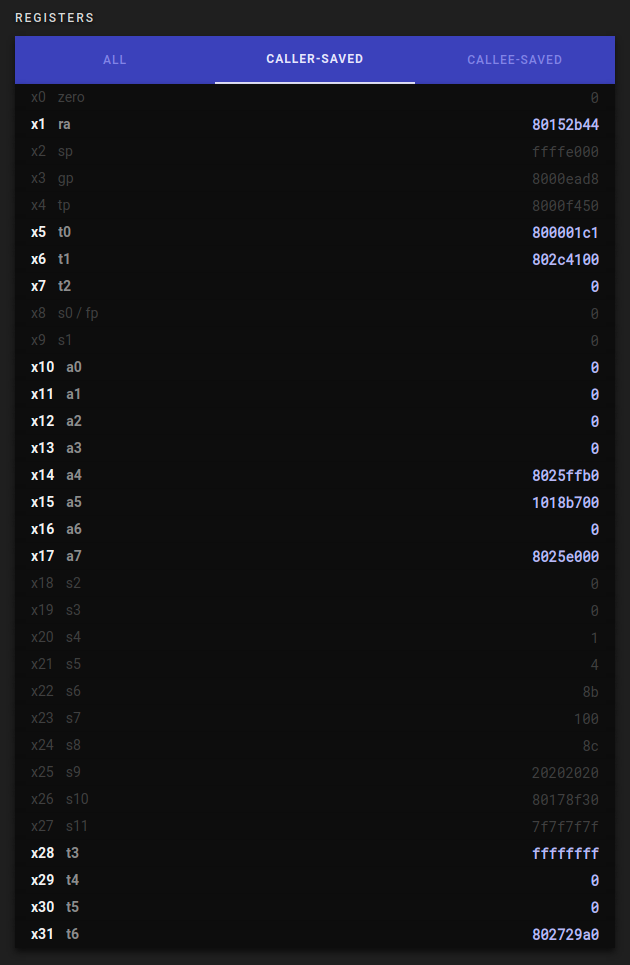
\includegraphics[scale=.35]{reg}
  \label{fig:reg}
  \caption{Register panel}
  \centering
\end{figure}

\noindent
the ratio of CPU instructions executed,

% change this when we have a picture of the prototype
\begin{figure}[H]
  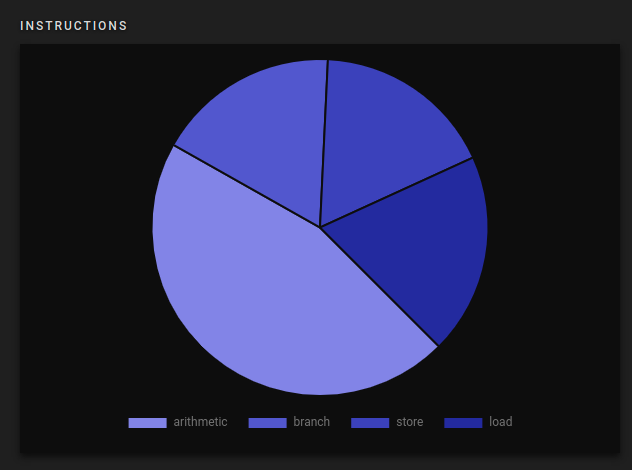
\includegraphics[scale=.4]{inst}
  \label{fig:inst}
  \caption{Instruction panel}
  \centering
\end{figure}

\noindent
and a time series graph showing memory utilization

% change this when we have a picture of the prototype
\begin{figure}[H]
  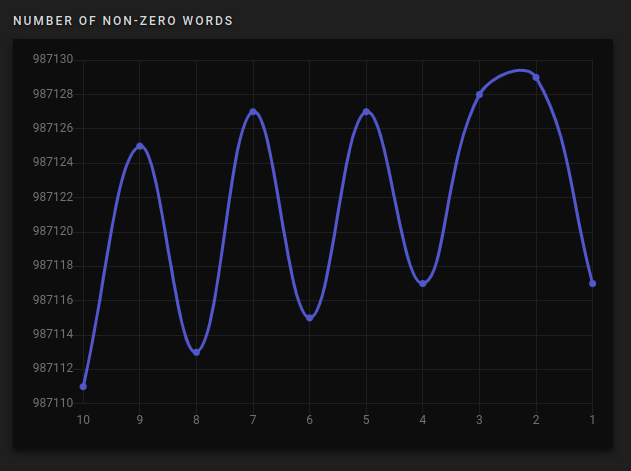
\includegraphics[scale=.4]{mem}
  \label{fig:mem}
  \caption{Memory panel}
  \centering
\end{figure}

\noindent
We feel that this offers a useful feature set to get a glance at what is going on under the hood
of an operating system utilizing the RISC-V instruction set.

% change this when we have a picture of the prototype
\begin{figure}[H]
  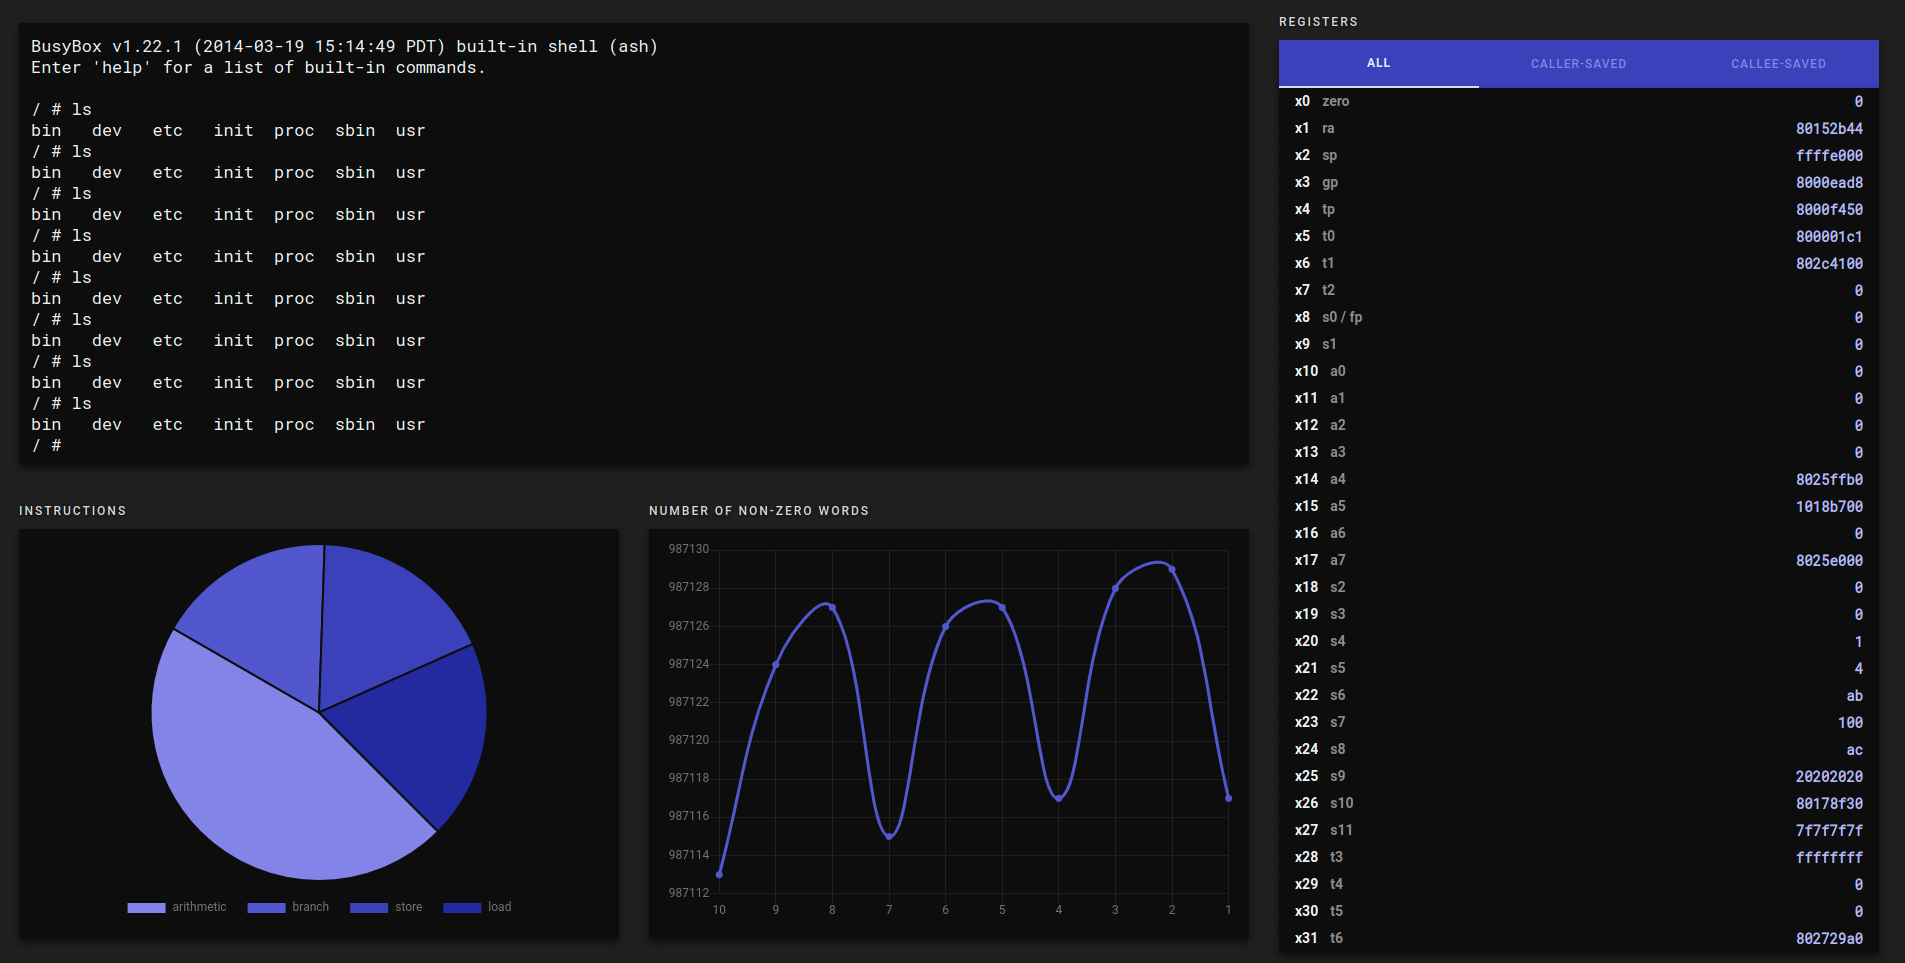
\includegraphics[scale=0.13]{dashboard}
  \label{fig:mvp}
  \caption{MVP}
  \centering
\end{figure}



%-------------------------------------------------------------------------------
\section*{Deployment}
%-------------------------------------------------------------------------------

After our prototype is complete, we prepare our application for deployment.
To keep things as simple as possible, we host the app on the
CSE department's servers at University of Washington. In this way, this project
can easily be used as an example in future iterations of the CSE481a capstone course.


%-------------------------------------------------------------------------------
\section*{Next Steps}
%-------------------------------------------------------------------------------

This project has a lot of room to grow. There are features still to be desired. Namely,

\begin{itemize}
  \item A way to see inside the file system
  \item A way to get information about running processes
\end{itemize}

We feel our project provides a modular foundation for these features to be developed in the future.
In hopes to reinvigorate life back into the riscv-angel project, we submitted a pull request
to merge our extensions into the base riscv-angel branch, from which this project is based on.



%-------------------------------------------------------------------------------
\section*{Conclusion}
%-------------------------------------------------------------------------------

In this project, we've taken an existing project, riscv-angel, and extended it to display
an interactive dashboard that lets users see the internals of an OS and CPU running on
a virtual machine.
We believe our project could be used by educators to easily show students properties of
an OS in real time.
We designed and developed this application with modularity in mind.
Our React component-based architecture allows features to rapidly developed and added to the UI.
We believe this application has the potential to reinvigorate interest in the original riscv-angel project.
At the very least, people can use our app to learn and experiment with an operating system running on a RISC-V architecture
with very little barrier to entry.


%-------------------------------------------------------------------------------
\section*{Acknowledgments}
%-------------------------------------------------------------------------------

Thanks to all of the contributors of \href{https://github.com/riscv/riscv-angel}{riscv-angel},
in which this project is based on.

%-------------------------------------------------------------------------------
\section*{Availability}
%-------------------------------------------------------------------------------

This project is open-source and is available at
\href{https://github.com/swkeever/riscv-angel-extended}
{https://github.com/swkeever/riscv-angel-extended}

%-------------------------------------------------------------------------------


%%%%%%%%%%%%%%%%%%%%%%%%%%%%%%%%%%%%%%%%%%%%%%%%%%%%%%%%%%%%%%%%%%%%%%%%%%%%%%%%
\end{document}
%%%%%%%%%%%%%%%%%%%%%%%%%%%%%%%%%%%%%%%%%%%%%%%%%%%%%%%%%%%%%%%%%%%%%%%%%%%%%%%%

%%  LocalWords:  endnotes includegraphics fread ptr nobj noindent
%%  LocalWords:  pdflatex acks
